\documentclass[tikz,border=3mm]{standalone}
\usetikzlibrary{positioning, shapes, fit}

\begin{document}
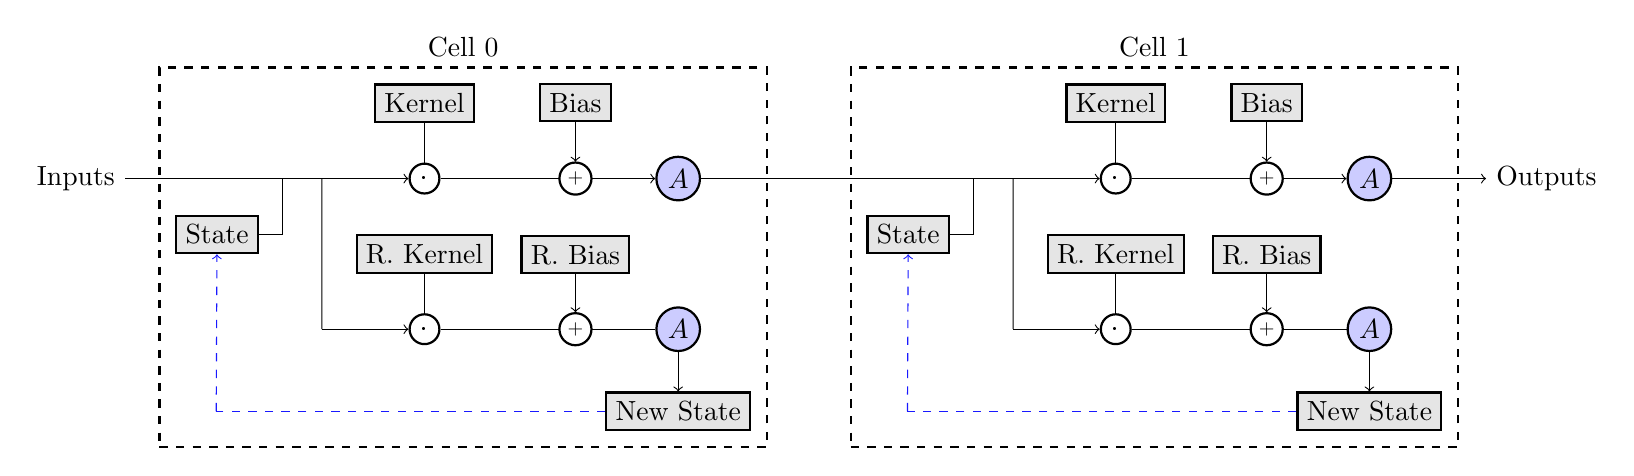
\begin{tikzpicture}[
    every node/.style={draw, thick},
    operation/.style={circle, inner sep=2pt},
    kernel/.style={rectangle, fill=gray!20},
    point/.style={coordinate},
    cell/.style={rectangle, draw, thick, dashed, inner sep=2mm, fit=#1}
]

% Cell 0

% output tree
\node[kernel] (c0_kernel) {Kernel};
\node[operation, below=5mm of c0_kernel] (c0_dot1) {·};
\node[operation, right=15mm of c0_dot1, scale=0.73] (c0_add1) {+};
\node[kernel, above=5mm of c0_add1] (c0_bias) {Bias};
\node[operation, right=8mm of c0_add1, fill=blue!20] (c0_activation1) {$A$};

% recur tree
\node[kernel, below=5mm of c0_dot1] (c0_recur_kernel) {R. Kernel};
\node[kernel, below=5mm of c0_add1] (c0_recur_bias) {R. Bias};
\node[operation, below=5mm of c0_recur_kernel] (c0_dot2) {·};
\node[operation, right=15mm of c0_dot2, scale=0.73] (c0_add2) {+};
\node[operation, right=8mm of c0_add2, fill=blue!20] (c0_activation2) {$A$};

\coordinate[left=16mm of c0_dot1] (c0_cat) {};
\coordinate[below=7.1mm of c0_cat] (c0_state_bridge) {};
\node[kernel, left=3mm of c0_state_bridge] (c0_state) {State};
\coordinate[right=5mm of c0_cat] (c0_sep) {};
\coordinate[left=5mm of c0_dot1] (c0_bridge1) {};
\coordinate[left=11mm of c0_dot2] (c0_bridge2) {};
\node[kernel, below=5mm of c0_activation2] (c0_new_state) {New State};
\coordinate[left=49.4mm of c0_new_state] (c0_new_state_bridge) {};

% Inputs and outputs
\node[rectangle, left=36mm of c0_dot1, draw=none] (input) {Inputs};

% output tree edges
\draw[->] (c0_kernel) -- (c0_dot1) -- (c0_add1) -- (c0_activation1);
\draw[->] (c0_bias) -- (c0_add1);

% recur tree edges
\draw[->] (c0_recur_kernel) -- (c0_dot2) -- (c0_add2) -- (c0_activation2) -- (c0_new_state);
\draw[->] (c0_recur_bias) -- (c0_add2);
\draw[-, dashed, draw=blue!90] (c0_new_state) -- (c0_new_state_bridge);
\draw[->, dashed, draw=blue!90] (c0_new_state_bridge) -- (c0_state);

% io cat edges
\draw[-] (input) -- (c0_cat);
\draw[-] (c0_state) -- (c0_state_bridge) -- (c0_cat) -- (c0_sep);
\draw[-] (c0_sep) -- (c0_bridge1);
\draw[-] (c0_sep) -- (c0_bridge2);
\draw[->] (c0_bridge1) -- (c0_dot1);
\draw[->] (c0_bridge2) -- (c0_dot2);

% Enclose cells
\node[cell=(c0_kernel)(c0_state)(c0_new_state), label=above:Cell 0] {};

% Cell 1
\node[kernel, right=75mm of c0_kernel] (c1_kernel) {Kernel};
\node[operation, below=5mm of c1_kernel] (c1_dot1) {·};
\node[operation, right=15mm of c1_dot1, scale=0.73] (c1_add1) {+};
\node[kernel, above=5mm of c1_add1] (c1_bias) {Bias};
\node[operation, right=8mm of c1_add1, fill=blue!20] (c1_activation1) {$A$};

% recur tree
\node[kernel, below=5mm of c1_dot1] (c1_recur_kernel) {R. Kernel};
\node[kernel, below=5mm of c1_add1] (c1_recur_bias) {R. Bias};
\node[operation, below=5mm of c1_recur_kernel] (c1_dot2) {·};
\node[operation, right=15mm of c1_dot2, scale=0.73] (c1_add2) {+};
\node[operation, right=8mm of c1_add2, fill=blue!20] (c1_activation2) {$A$};

\coordinate[left=16mm of c1_dot1] (c1_cat) {};
\coordinate[below=7.1mm of c1_cat] (c1_state_bridge) {};
\node[kernel, left=3mm of c1_state_bridge] (c1_state) {State};
\coordinate[right=5mm of c1_cat] (c1_sep) {};
\coordinate[left=5mm of c1_dot1] (c1_bridge1) {};
\coordinate[left=11mm of c1_dot2] (c1_bridge2) {};
\node[kernel, below=5mm of c1_activation2] (c1_new_state) {New State};
\coordinate[left=49.4mm of c1_new_state] (c1_new_state_bridge) {};

% output tree edges
\draw[->] (c1_kernel) -- (c1_dot1) -- (c1_add1) -- (c1_activation1);
\draw[->] (c1_bias) -- (c1_add1);

% recur tree edges
\draw[->] (c1_recur_kernel) -- (c1_dot2) -- (c1_add2) -- (c1_activation2) -- (c1_new_state);
\draw[->] (c1_recur_bias) -- (c1_add2);
\draw[-, dashed, draw=blue!90] (c1_new_state) -- (c1_new_state_bridge);
\draw[->, dashed, draw=blue!90] (c1_new_state_bridge) -- (c1_state);

% io cat edges
\draw[-] (c0_activation1) -- (c1_cat);
\draw[-] (c1_state) -- (c1_state_bridge) -- (c1_cat) -- (c1_sep);
\draw[-] (c1_sep) -- (c1_bridge1);
\draw[-] (c1_sep) -- (c1_bridge2);
\draw[->] (c1_bridge1) -- (c1_dot1);
\draw[->] (c1_bridge2) -- (c1_dot2);

% Enclose cells
\node[cell=(c1_kernel)(c1_state)(c1_new_state), label=above:Cell 1] {};

% Output
\node[rectangle, right=45mm of c1_dot1, draw=none] (output) {Outputs};
\draw[->] (c1_activation1) -- (output);

\end{tikzpicture}
\end{document}
